\chapter{基于多核学习的浮游生物图像分类研究}

使用多核学习融合多种不同特征可以更好的发挥每种特征在分类过程中的积极作用。本章首先对多核学习的理论进行介绍;然后介绍设计的分类系统;最后,设计一系列对比实验分析分类系统的性能,并根据实验结果对分类系统性能进行评价。

\section{多核学习理论}

在图像分类识别过程中采用多种特征对目标进行描述有利于提高分类的准确率,而在这个过程中如何融合多种特征的方法又是人们关注的重点。通常特征融合算法可以分为决策级融合、特征级融合和数据级融合三类。数据级融合是将未加工的图像信息结合来得到更丰富的信息,常用的算法有主成分分析、线性加权法等。特征级融合是通过选择去除多余的特征,然后融合不相关的特征,例如聚类分析法、信息熵法等。决策级融合是将多个分类器结合,常用算法有贝叶斯融合、模糊聚类法、多核学习算法等。在本文中使用多核学习算法对提取的多种特征进行融合并训练分类器。

多核学习属于多视角学习。我们经常使用的支持向量机是一种单核学习方法,往往不能满足处理多种特征的需求,而多核学习为融合几种不同的核进行训练的学习方法,可以充分发挥每种特征在分类过程中的积极作用。下面以支持向量机为基础介绍核函数的原理,进而介绍多核学习的理论和方法。

\subsection{支持向量机}

早在1995年Cortes等人提出了支持向量机(Support Vector Machine, SVM)~\cite{Cortes1995Support},该方法属于监督学习,常用于目标分类和回归分析。支持向量机以VC维理论和结构风险最小化原理为基础,基本思想是在特征空间中构建一个最大间隔分类超平实现对未知样本的分类。因此,该方法适合处理二分类和回归问题,被普遍的应用在统计分类和回归分析中。

\subsubsection{线性可分支持向量机}

线性可分支持向量机是指训练样本在特征空间中线性可分,可以找到一个线性超平面将不同类别的样本完全正确的分开。设给定的样本为$(x_{1},y_{1}),\cdots,(x_{n},y_{n})$,其中$x_{i}\in X = R^{n}$,$y_{i}\in \{1,-1\}$,$x_{i}$为第$i$个样本的特征向量,$y_{i}$为第$i$个样本所属的类别。支持向量机对样本进行分类是通过在特征空间中找到最大间隔超平面将不同类别的样本划分开,如图~\ref{fig:svm}所示,超平面的方程可以表示为:
\begin{figure}%[H] % use float package if you want it here
  \centering
  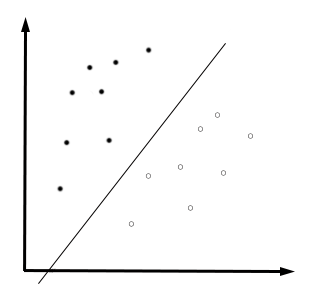
\includegraphics[height=4cm]{MKL/svm}
  \caption{SVM分类超平面}
  \label{fig:svm}
\end{figure}
\begin{eqnarray}
w^{T}x+b=0
\end{eqnarray}
其中,$w$表示垂直于超平面的向量,$b$表示超平面的截距,该分类问题的决策函数为:
\begin{eqnarray}
f(x)=s(w^{T}x+b)
\end{eqnarray}
若$f(x_{i})$大于0,则$x_{i}$为类别$1$,否则为类别$-1$。

若要找到最大间隔超平面,则需要计算样本到超平面的距离。通常$|wx_{i}+b|$可以表示样本点$i$距离超平面的远近,而$wx_{i}+b$与$y_{i}$的符号相同,因此可以用$\hat{\gamma}=y(wx+b)$表示样本到分类平面的距离,这就是函数间隔。然而在选择超平面时,$w$和$b$等比例的变化并不会改变超平面,但是却会改变函数间隔。因此,引入几何间隔:
\begin{eqnarray}
\tilde{\gamma}=\frac{\hat{\gamma}}{||w||}
\end{eqnarray}

一个超平面的几何间隔是所有训练样本距离该超平面的几何间隔中的最小值,而支持向量机得学习目标是要在特征空间中找到一个超平面,使其几何间隔最大。对线性可分的样本集来说,其线性可分超平面有很多个,然而几何间隔最大的分类超平面就一个。

若要找到最大间隔分类超平面,需要令几何间隔最大,即:
\begin{eqnarray}
\max \tilde{\gamma}=\max\frac{\hat{\gamma}}{||w||}=\max\frac{y(w^{T}x+b)}{||w||}
\end{eqnarray}

其中函数间隔$\hat{\gamma}$的大小并不会对上述最优化问题造成影响,因此令$\hat{\gamma}=1$,将其代入\ref{equ:chap4:youhua},并且最大化$\frac{1}{||w||}$和最小化$\frac{1}{2}||w||$是等价的,得到求解支持向量机的最优化问题为:
\begin{eqnarray}
\min\frac{1}{2}||w||^{2},~~~s.t. ~~ y_{i}(w^{T}x_{i}+b) \ge 1, i=1,\cdots,n
\end{eqnarray}
可以将上述最优化问题看做其原始问题,求解其对偶问题可以获得最优解。首先构建拉格朗日函数:
\begin{eqnarray}
\label{equ:chap4:youhua}
L(w,b,\alpha)=\frac{1}{2}||w||^{2}-\sum^{n}_{i=1}\alpha_{i}[y_{i}(w^{T}x_{i}+b)-1]
\end{eqnarray}
按照拉格朗日对偶性,原始问题可以转换为对偶问题的极大极小问题,即:
\begin{eqnarray}
\min_{w,b}\theta(w)=\min_{w,b}\max_{\alpha_{i}\ge 0}L(w,b,\alpha)
\end{eqnarray}
求解以上对偶问题首先要固定$\alpha$求$L(w,b,\alpha)$关于$w,b$的极小,然后求对$\alpha$的极大,就可以得到与之等价的对偶优化问题:
\begin{eqnarray}
\min_{\alpha}\frac{1}{2}\sum^{n}_{i=1}\sum^{n}_{j=1}\alpha_{i}\alpha_{j}y_{i}y_{j}<x_{i}\cdot x_{j}>-\sum^{n}_{i=1}\alpha_{i}\\
s.t. ~~~ \sum^{n}_{i=1}\alpha_{i}y_{j}=0\\
\alpha_{i} \ge 0, i=1,2,\cdots,n
\end{eqnarray}

在KKT条件成立的前提下,可以得到:
\begin{eqnarray}
w = \sum^{n}_{i=1}\alpha_{i}y_{i}x_{i}
\end{eqnarray}
\begin{eqnarray}
b = y_{j}-\sum^{n}_{i=1}\alpha_{i}y_{i}<x_{i}\cdot x{j}>
\end{eqnarray}

由此可以得到分类超平面和决策函数分别为:
\begin{eqnarray}
\sum^{n}_{i=1}\alpha_{i}y_{j}<x\cdot x_{i}>+b=0
\end{eqnarray}
\begin{eqnarray}
f(x)=s(\sum^{n}_{i=1}\alpha_{i}y_{i}<x_{i},x>+b)
\end{eqnarray}

\subsubsection{线性不可分支持向量机}

对于分类中遇到线性不可分情况,需要把原始的特征映射到高维空间中,采用非线性变换将它转换为高维空间中的线性可分问题。假设低维空间的数据到高维空间的映射为$\phi$,则式~\ref{equ:chap4:youhua}可以转化为:
\begin{eqnarray}
L(w,b,\alpha)=\sum^{n}_{i=1}\alpha_{i}-\frac{1}{2}\sum^{n}_{i,j=1}\alpha_{i}\alpha_{j}y_{i}y_{j}\phi(x_{i})\cdot\phi(x_{j})
\end{eqnarray}

由于非线性映射比较复杂,因此引入核函数计算两个向量在映射到高维空间的内积函数:
\begin{eqnarray}
K(x_{i},x_{j})=\phi(x_{i})\cdot\phi(x_{j})
\end{eqnarray}

这样在对样本点进行预测时,只需要计算其在高维空间中的内积。引入核函数后,不必知道低维空间到高维空间映射$\phi$的具体形式,能够根据原空间的函数计算得到内积。优化问题中引入核函数可得:
\begin{eqnarray}
L(w,b,\alpha)=\sum^{n}_{i=1}\alpha_{i}-\frac{1}{2}\sum^{n}_{i,j=1}\alpha_{i}\alpha_{j}y_{i}y_{j}K(x_{i},x_{j})
\end{eqnarray}

同样可以得到决策函数为:
\begin{eqnarray}
f(x)=s(\sum^{n}_{i=1}\alpha_{i}y_{i}K(x_{i},x_{j})+b)
\end{eqnarray}

\subsection{核函数}

核函数理论出现的较早,可以追溯到1909年的Mercer定理和之后再生核希尔伯特空间的出现。后来人们在研究势函数时将核函数应用到机器学习领域,之后核函数在将线性支持向量机推广到非线性支持向量机时充分发挥了作用。

支持向量机在处理线性不可分的问题时,使用核函数将低维空间中的数据转换到高维空间中,通过在高维特征空间中建立超平面把样本区分开,从而实现将线性不可分问题转换成高维空间中的线性可分问题。在这个过程中,无需知道数据在高维空间中的具体形式,既避免“维数灾难”等问题的发生,也减少了计算的复杂度。

\begin{definition}
核函数:设$\chi$是输入空间,$H$为希尔伯特空间,如果存在一个从$\chi$到$H$的映射$\phi:\chi\to H$,使得对所有$x_{i},x_{j}\in \chi$,函数$K(x_{i},x_{j})$满足条件
\begin{gather*}
\begin{split}
K(x_{i},x_{j})=\phi(x_{i})\cdot\phi(x_{j})
\end{split}
\end{gather*}
则称$K(x_{i},x_{j})$为核函数。
\end{definition}

使用核函数的优点是在训练分类器过程中,不需要知道$\phi$的具体形式,可以直接使用核函数进行计算。目前比较常用的核函数有以下几种:
\begin{enumerate}
\item 线性核函数:
	\begin{eqnarray}
	k(x_{1},x_{2})=<x_{1},x_{2}>
	\end{eqnarray}
\item 多项式核函数:是采用$n$阶多项式实现。
	\begin{eqnarray}
	k(x_{1},x_{2})=(\gamma<x_{1},x_{2}>+R)^{n}
	\end{eqnarray}
\item 高斯径向基核函数:是最常用的核函数,可以把低维空间中的数据映射到无穷维。
	\begin{eqnarray}
	k(x_{1},x_{2})=e^{-\gamma||x_{1}-x_{2}||^{2}}
	\end{eqnarray}
\item Sigmoid核函数:
	\begin{eqnarray}
	k(x_{1},x_{2})=\tanh(\gamma<x_{1},x_{2}>+R)
	\end{eqnarray}
\end{enumerate}

\subsection{多核学习}

\subsubsection{多核学习原理}

支持向量机是基于单核的分类算法,使用同一个核函数处理所有特征数据。然而不一样的核函数反应着的映射关系是不同的,因此针对不同数据使用不一样的核函数得到的分类效果会有一定差异。然而,在处理实际分类问题时,针对一幅图像提取一种特征往往是不够的,需要提取多种特征。显然,这时采用单个核函数并不能实现对所有特征的最优映射,在这种情况下,采用多个核函数比一个核函数更有助于提高分类的准确率。多核学习为每类特征指定核函数,给每个核赋予适合的权重,然后将所有的核函数组合到一起。在这个过程中,多核学习的研究重点是如何选择基本核及其权重。

构造多核学习模型的过程就是为每类特征选定合适的基本核,然后将它们组合到一起形成合成核。多核学习算法结构如图~\ref{fig:MKL}所示。从图中可以看出,对于输入的数据中的不同特征分别为其选定适合的核函数,计算每个核函数的对应权重,按照一定的规则结合到一起形成合成核。合成核的基本形式为:
\begin{eqnarray}
K(x_{i},x_{j})=f({k_{m}(x^{m}_{i},x^{m}_{j})}^{P}_{m=1})
\end{eqnarray}
其中$k_{m}(x_{i},x_{j})$是基本核函数;$m$表示使用的基本核数量;$f$表示核结合函数,它决定基本核函数的结合形式,可以是线性或非线性函数。
\begin{figure}[H] % use float package if you want it here
  \centering
  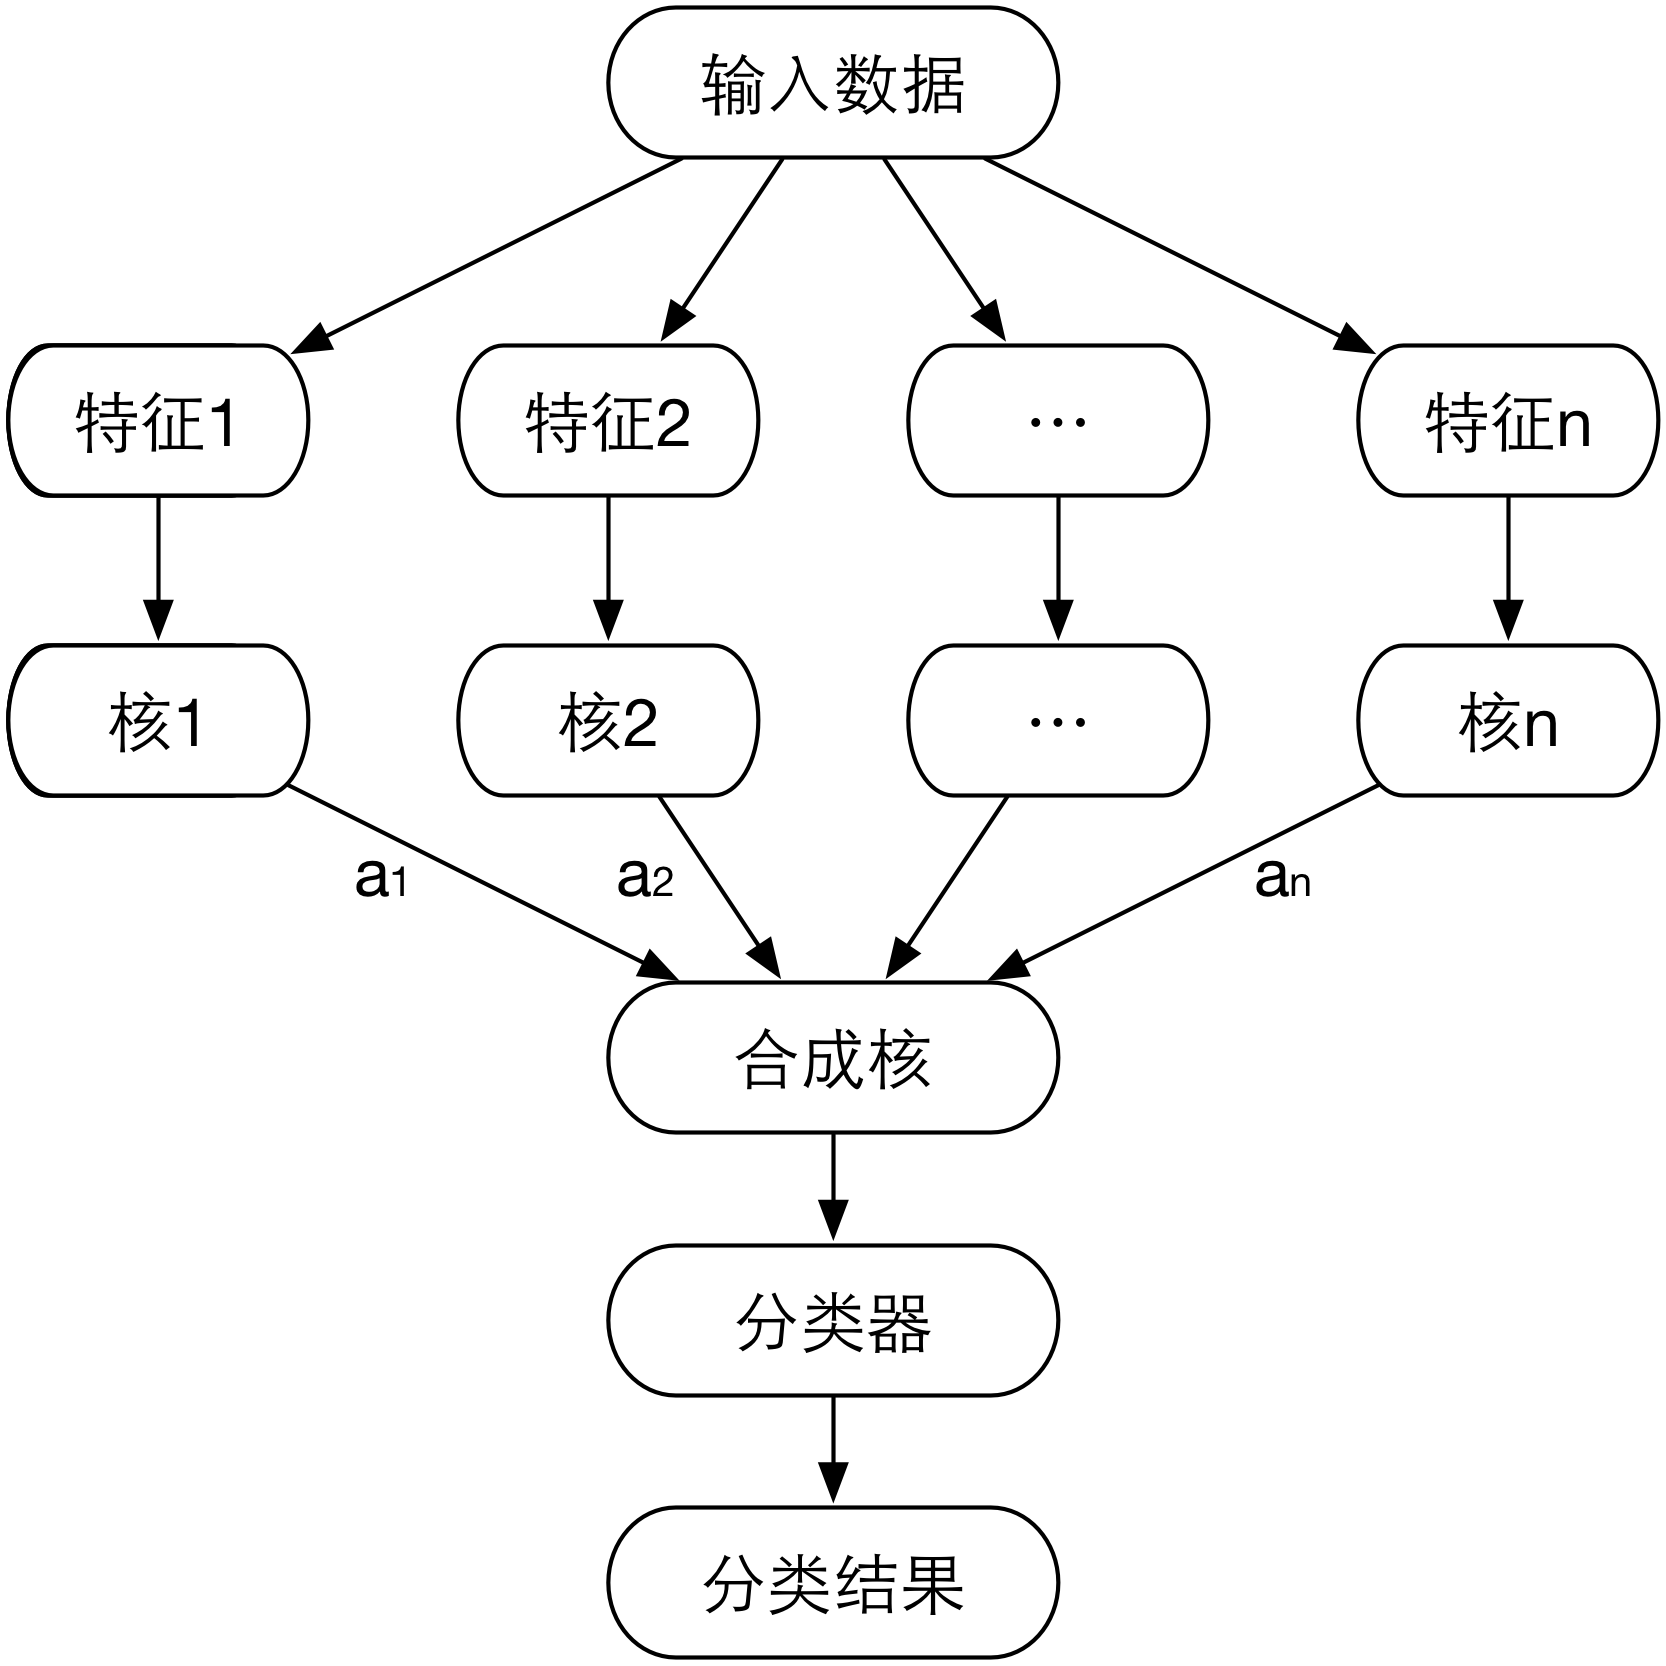
\includegraphics[height=7cm]{MKL/MKL}
  \caption{多核学习算法结构}
  \label{fig:MKL}
\end{figure}


% 确定上述判别函数通过解以下二次优化问题实现:
% \begin{eqnarray}
% \left\{ \begin{array}{l} \min \frac{1}{2}||w||^{2}_{2}+C\sum^{N}_{i=1}\xi_{i}\\
% w \in R^{s}, \xi \in R^{N}_{+}, b \in R\\
% y_{i}(<w,\phi(x_{i})>+b) \ge 1-\xi_{i} ~~~ \forall i \end{array} \right.
% \end{eqnarray}
% 其中,$w$是向量的权重,$C$为惩罚因子,$\xi$为松弛变量,$b$为超平面的偏置项。以上最优化问题并不是直接解,而是通过拉格朗日变换转化为对偶问题:
% \begin{eqnarray}
% \left\{ \begin{array}{l} \max\sum^{n}_{i=1}\alpha_{i}-\frac{1}{2}\sum^{n}_{i,j=1}\alpha_{i}\alpha_{j}y_{i}y_{j}\underbrace{< \phi(x_{i}),\phi(x_{j}) >}_{k(x_{i},x_{j})}\\
% \alpha \in R^{N}_{+}\\
% \sum^{N}_{i=1}\alpha_{i}y_{i}=0\\
% C \ge \alpha_{i} \ge 0 ~~~ \forall i\end{array} \right.
% \end{eqnarray}
% 上式中$k$为核函数。将上式代入到判别函数中可以得到:
% \begin{eqnarray}
% f(x)=\sum^{N}_{i=1}\alpha_{i}y_{i}k(x,x_{i})+b
% \end{eqnarray}



多核学习有六个关键属性:(1)确定结合函数的方法,(2)结合核函数的形式,(3)确定结合函数参数的目标函数形式,(4)计算结合函数参数的训练方法,(5)基本学习算法,(6)多核学习的计算复杂度。根据上述不同属性可以将多核学习算法进行分类~\cite{gonen2011multiple}:
\begin{enumerate}
\item 现有的多核学习算法用不同的学习方法来确定核结合函数的形式,根据方法的不同可以将这些算法分为5类:固定形式结合方法、启发式方法、最优化方法、贝叶斯方法和Boosting方法。
  \begin{itemize}
  \item 固定形式是指结合函数中没有任何参数,不需要训练,例如将核以固定的形式相加或相乘。
  \item 启发式方法采用有参数的结合函数组合基本核,根据核矩阵或每个核单独使用时的表现来确定函数的参数。
  \item 最优化方法也是使用有参数的结合函数,通过解最优化问题来确定参数。
  \item 贝叶斯方法将核结合函数的参数看做随机值,先设定这些参数先验值,然后通过推理学习参数。
  \item Boosting方法的思想来源于集成学习,通过迭代增加新的核直到分类性能不再提高为止。
  \end{itemize}
\item 多核学习算法根据核函数融合方式不同可以将其分为:线性结合、非线性结合和数据依赖结合。
  \begin{itemize}
  \item 线性结合是目前应用较广的方法,主要包括无权重求和和有权重求和两种。
  \item 非线性结合方法是指使用非线性函数做为结合函数,例如包含相乘、幂运算的函数。
  \item 数据依赖结合是指定特定的核权重给每组数据,学习每个区域中最优核结合方式。
  \end{itemize}
\item 确定结合函数参数能够根据优化不同目标函数得到,现有的目标函数一般分为三类:相似性函数、结构风险函数和贝叶斯函数。
  \begin{itemize}
  \item 相似性目标函数是通过最大化相似度来确定结合函数的参数(相似度是根据训练集计算出结合核矩阵和最优核矩阵之间的相似性)。
  \item 结构风险函数根据最小化正则项和误差项之和来确定结合函数的参数,这称之为结构风险最小化。
  \item 贝叶斯函数是用贝叶斯公式计算结合核的参数。
  \end{itemize}
\item 计算结合函数参数的训练方法包括两种。一种是直接计算出结合函数参数和基础核函数参数;另一种是通过迭代的方法实现,先固定基础核函数的参数,更新结合函数的参数,然后再固定结合函数的参数,更新基础核函数的参数,直到最终收敛就完成了训练。
\item 多核学习的基础学习算法有很多,例如支持向量机、核Fisher判别分析、核岭回归等。
\item 多核学习的计算复杂度主要依赖于训练方法和基础学习方法的复杂度。
\end{enumerate}

同支持向量机这样的单核学习算法相比,多核学习在训练中不仅要计算w,b的值,还要得到每个核函数的权重。在这里最重要的问题是如何确定权重,近年来许多多核学习算法都是针对这一问题提出的。

多核学习算法中最经典的方法是简单多核学习(SimpleMKL)~\cite{rakotomamonjy2008simplemkl},它被看做为多核学习算法的具体实现。后来人们还提出了广义多核学习(Generalized Multiple Kernel Learning, GMKL)~\cite{varma2009more}、局部多核学习(Localized Multiple Kernel Learning, LMKL)~\cite{gonen2008localized}、非线性多核学习(Non-Linear Multiple Kernel Learning, NLMKL)~\cite{cortes2009learning}等算法,下面对简单多核学习和本文中使用的非线性多核学习算法进行介绍。

\subsubsection{简单多核学习}
SimpleMKL~\cite{rakotomamonjy2008simplemkl}使用线性结合的方式将多个基础核函数组合得到一个新的核函数,并采用梯度下降法求解,其核函数形式为:
\begin{eqnarray}
K(x_{i},x_{j})=\sum^{M}_{m=1}d_{m}k_{m}(x_{i},x_{j}), ~~~ with ~ d_{m} \ge 0, ~\sum^{M}_{m=1}d_{m}=1
\end{eqnarray}
上式中,$k_{m}$表示基础核函数,$M$表示基础核函数的数量,$d_{m}$是基础核函数对应的权重系数,它表示着特征在分类过程中的重要性,是多核学习过程中需要求解的重要问题。根据支持向量机的原理,SimpleMKL的原始优化问题可以等价为如下凸优化问题~\cite{孙锐2014基于多特征和多核学习的行人检测方法的研究}:
\begin{eqnarray}
\left\{ \begin{array}{l} \min \frac{1}{2}\sum_{m}\frac{1}{d_{m}}||f_{m}||^{2}+C\sum_{i}\xi_{i}\\
s.t ~~~ y_{i}\sum^{M}_{m=1}f_{m}(x_{i})+y_{i}b \ge 1-\xi ~~~ \forall i\\
\xi_{i}\ge 0 ~~~ \forall i\\
\sum^{M}_{m=1}d_{m}=1, ~~~ d_{m} \ge 0 ~~ \forall m\end{array} \right.
\end{eqnarray}
上式中,$f_{m}$为希尔伯特空间中的分类超平面。该式为多核学习的原始问题,要根据其确定参数$d_{m}$。采用拉格朗日算法可以将上述原始优化问题转换成对偶问题得到:
\begin{multline}
L=\frac{1}{2}\sum_{m}\frac{1}{d_{m}}||f_{m}||^{2}+C\sum_{i}\xi_{i}+\sum_{i}\alpha_{i}(1-\xi_{i}-y_{i}\sum_{m}f_{m}(x_{i})-y_{i}b)\\
-\sum_{i}v_{i}\xi_{i}+\lambda(\sum_{m}d_{m}-1)-\sum_{m}\eta_{m}d_{m}
\end{multline}
其中$\alpha_{i}$和$v_{i}$为拉格朗日乘子,而$\lambda$和$\eta_{m}$表示权重$d_{m}$的约束。接着分别对$L$自变量求偏导数,并令导数为0可得:%$f_{m},b,\xi_{m},d_{m}$
\begin{eqnarray}
\left\{ \begin{array}{l}\frac{1}{d_{m}}f_{m}(\bullet)=\sum_{i}\alpha_{i}y_{i}K_{m}(\bullet,x_{i}), ~~~ \forall m\\
\sum_{i}\alpha_{i}y_{i}=0\\
C-\alpha_{i}-v_{i}=0, ~~~ \forall i\\
-\frac{1}{2}\frac{||f_{m}||^{2}}{d^{2}_{m}}+\lambda-\eta_{m}=0, ~~~ \forall m\end{array} \right.
\end{eqnarray}

采用拉格朗日得到的对偶问题由于持续约束难以优化,这种约束可能转移到目标函数,但是目标函数变为不可微的,同样会造成求解困难。SimpleMKL带约束的优化问题为:
\begin{eqnarray}
\min_{d}J(d) ~~ s.t. \sum^{M}_{m=1}d_{m}=1,d_{M}\ge 0\\
J(d)=\left\{\begin{array}{l}\min_{{f},b,\xi}\frac{1}{2}\sum_{m}\frac{1}{d_{m}}||f_{m}||^{2}+C\sum_{i}\xi_{i} ~~~ \forall i\\
s.t. ~~~ y_{i}\sum_{m}f_{m}(x_{i})+y_{i}b \ge 1-\xi_{i}\\
\xi_{i}\ge 0 ~~~ \forall i\end{array}\right.
\end{eqnarray}

将上式可以转化为对偶问题:
\begin{eqnarray}
J(d)=-\frac{1}{2}\sum_{i,j}\alpha_{i}\alpha_{j}y_{i}y_{j}\sum{m}d_{m}K_{m}(x_{i},x_{j})+\sum_{i}\alpha_{i}
\end{eqnarray}

采用梯度下降法计算$J(d)$的梯度下降表示,不断的更新$d$的值直到满足停止准则。根据支持向量机求解原理,SimpleMKL的决策函数为:
\begin{eqnarray}
f(x)=s(\sum^{N}_{i=1}\sum^{M}_{m=1}d_{m}\alpha_{i}y_{i}K_{m}(x_{i},x_{j})+b)
\end{eqnarray}

\subsubsection{非线性多核学习}

上面介绍的简单多核学习得到的分类器性能要比使用单个核的支持向量机好,该方法实质上可以看成支持向量机使用多个不同核函数的线性组合。Gonen等人在2011发表的文章~\cite{gonen2011multiple}中对多种多核学习算法的性能进行了分析,他们在多个数据集上进行实验发现,采用非线性多核学习更有利于改善分类的性能。本文设计的浮游生物分类系统正是使用了非线性多核学习进行特征融合和训练分类器。Cortes等人~\cite{cortes2009learning}提出了非线性多核学习(Non-linear Multiple Kernel learning, NLMKL),该方法基于核岭回归(Kernel ridge regression, KRR)采用多项式函数将核进行融合,他们提出的结合核的形式如下:
\begin{eqnarray}
K_{\eta}(x_{i},x_{j})=\sum_{q\in Q}\eta_{q_{1}q_{2}\cdots q_{m}}k_{1}\cdots k_{m}
\end{eqnarray}
其中$Q=\{q:q\in Z^{m}_{+}, \sum^{m}_{l=1}q_{l}\le d\}$。然而上式中需要学习的参数较多,为了减少学习的复杂度,将其化简为:
\begin{eqnarray}
K_{\eta}(x_{i},x_{j})=\sum_{q\in R}\eta^{q_{1}}_{1}\eta^{q_{2}}_{2}\cdots\eta^{q_{m}}_{m}k_{1}\cdots k_{m}
\end{eqnarray}
其中$R=\{q:q\in Z^{m}_{+}, \sum^{m}_{l=1}q_{l}=d\}$。例如,当$d=2$时,核函数为:
\begin{eqnarray}
K_{\eta}(x_{i},x_{j})=\sum^{m}_{l=1}\sum^{m}_{h=1}\eta_{l}\eta_{h}k_{l}k_{h}
\end{eqnarray}

在该非线性多核学习中,结合核函数的权重通过解最小-最大优化问题来求得。\\


在浮游生物的分类识别过程中为了提高分类的准确度通常要融合多种特征。在遇到多种特征进行分类的问题时,只采用单个核函数进行分类并不能充分发挥每种特征的作用。多核学习是通过为每种特征选择分别选择核函数并融合在一起来构建分类器,这种方法可以有效的处理特征并解决单一核函数存在的不足。本文中我们使用非线性多核学习~\cite{cortes2009learning}来设计浮游生物分类系统,下面该分类系统进行详细介绍。

\section{基于多核学习的浮游生物图像分类系统}
\label{sec:system}

我们研究浮游生物自动分类系统的出发点是扩大其适用范围,提高分类性能。因此在设计分类系统时采用多种特征提取方法对浮游生物形态特征进行描述,并结合了特征选择和多核学习方法来构建分类模型。本文提出的浮游生物自动分类系统由以下四个部分组成:图像预处理、特征提取、特征选择、多核学习,其算法结构流程图如图~\ref{fig:frame}所示。
\begin{figure}[H] % use float package if you want it here
  \centering
  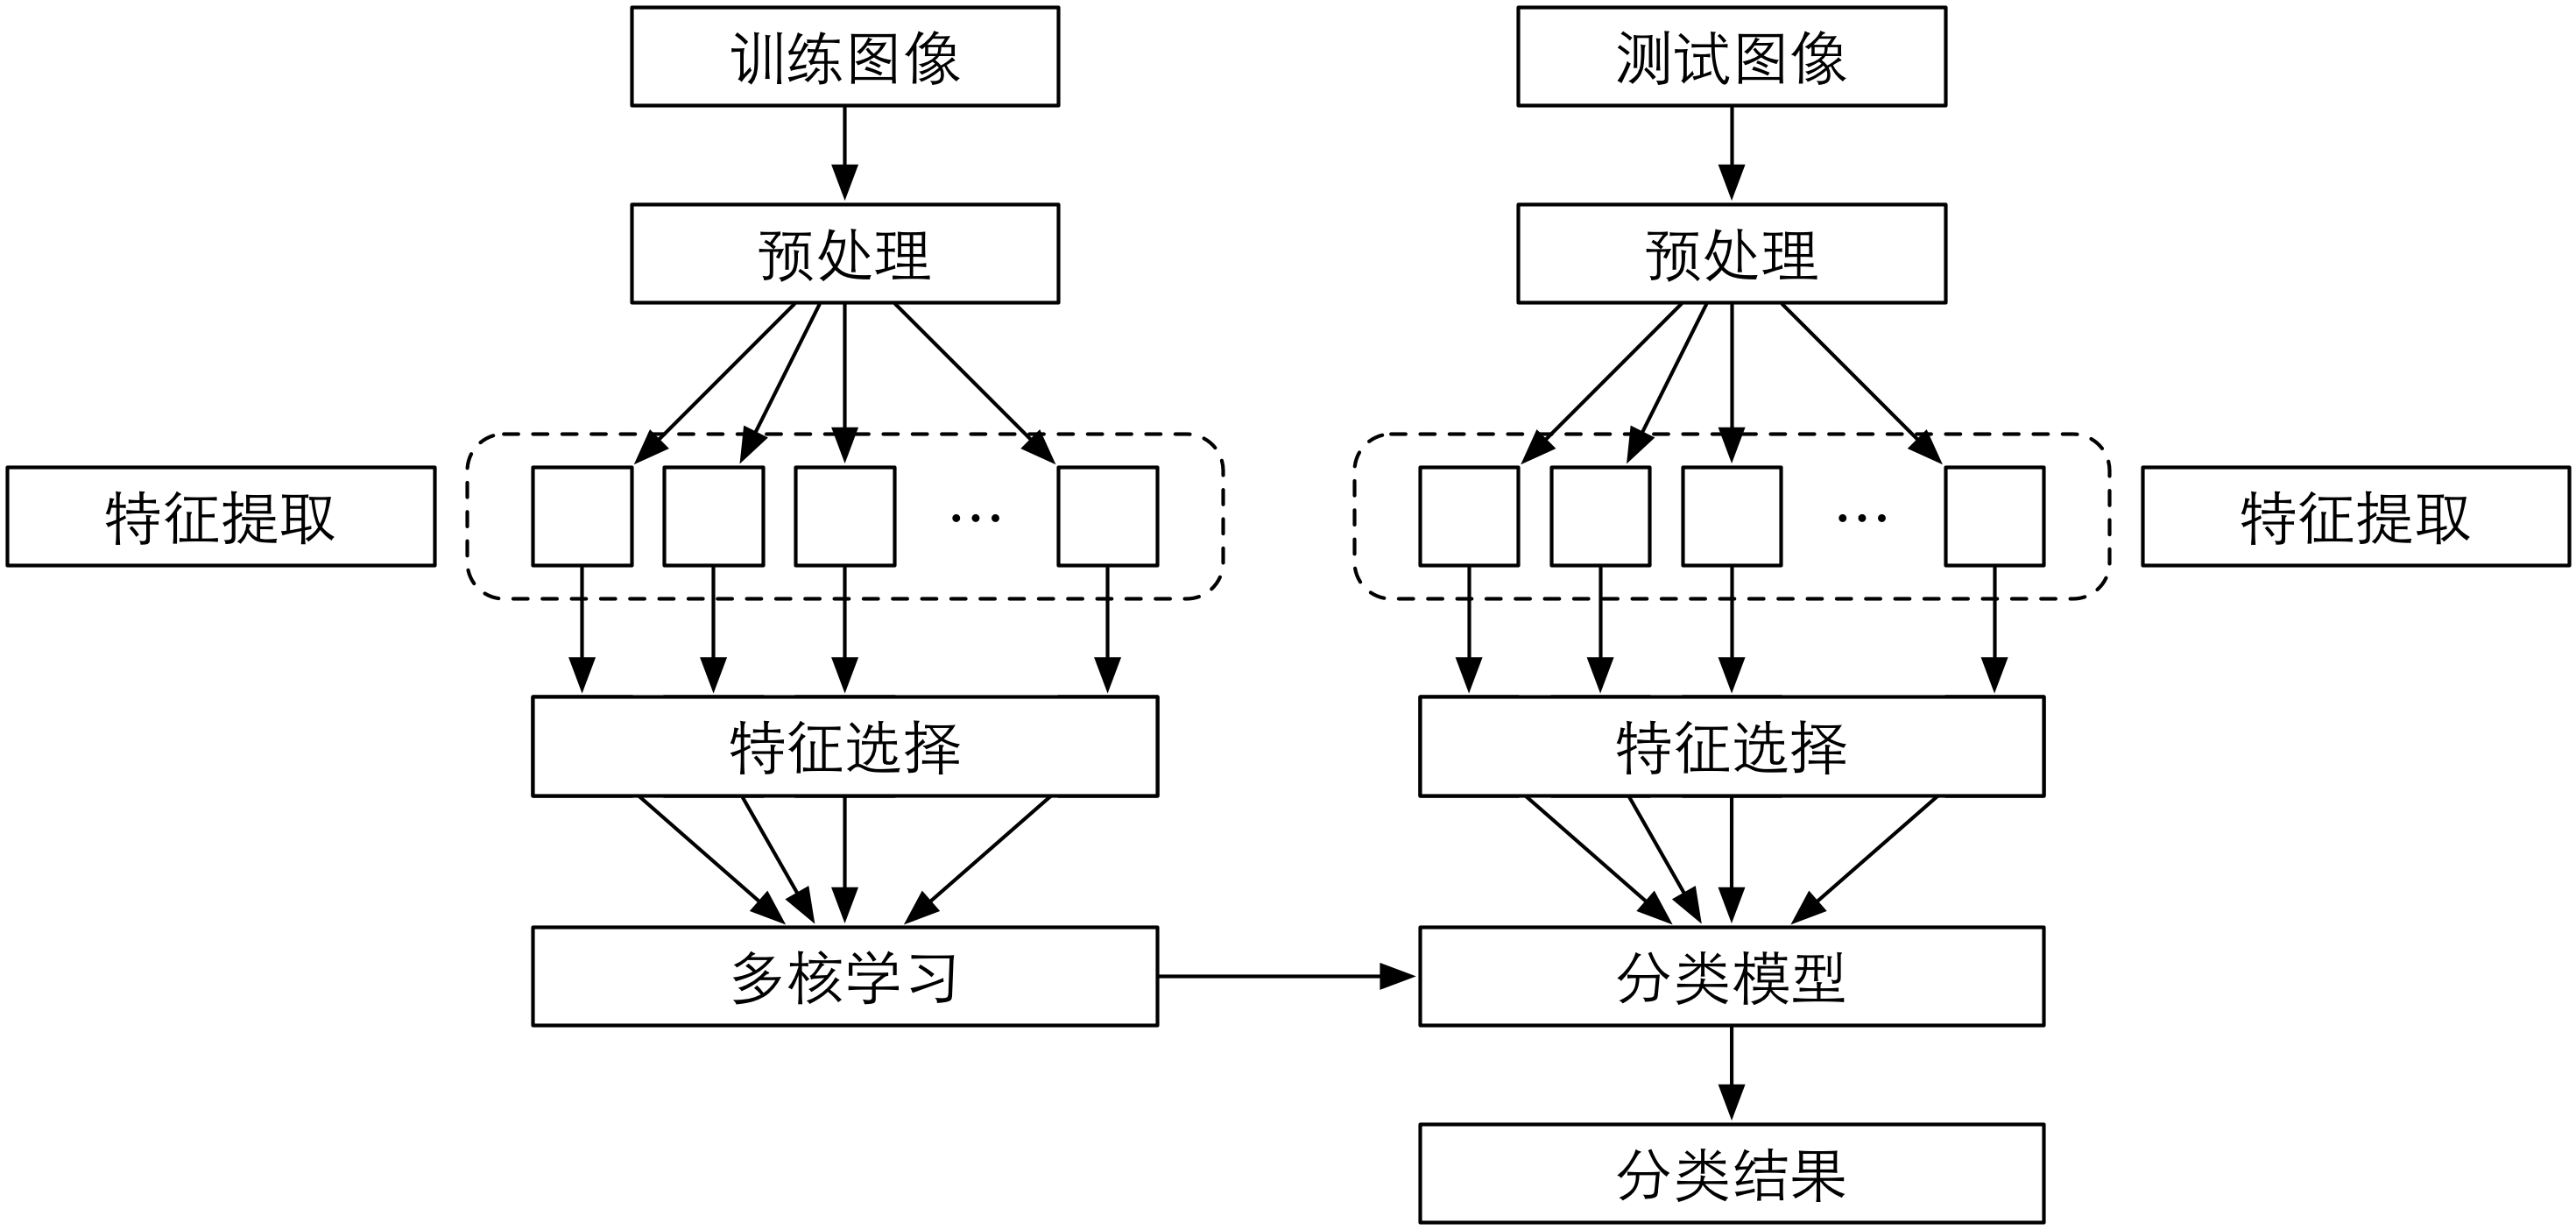
\includegraphics[height=6cm]{frame}
  \caption{基于多核学习的浮游生物分类系统算法结构流程图}
  \label{fig:frame}
\end{figure}

1、图像预处理

图像预处理是在图像识别之前进行的准备工作,包括去除图中的噪声、二值化分割图像背景等处理,避免无关因素对之后分类的影响。浮游生物数据集中的图像由水下图像采集设备获得,在采集浮游生物图像的过程中不可避免的会受到水中杂质等因素的干扰,造成采集的图像中会含悬浮物等噪声。因此为了提高图像的质量,在进行特征提取前要对采集的浮游生物图像进行预处理。

在本文实验使用的三个数据集中,WHOI采集的浮游生物图像没有分割,因此在预处理时首先要对该数据集进行分割。对该数据集的图像通过检测边缘进行分割~\cite{sosik2007automated}:首先将灰度图像进行相位一致性计算,然后采用Canny算子检测图像中的边缘,将获得的边缘图像用数学形态学算法(闭运算、膨胀、细化)进行处理,得到简单的轮廓边缘,使用获得的轮廓边缘就可以对其对应的浮游生物图像进行分割。

由于原浮游生物图像中可能存在悬浮颗粒等杂质,分割后图像中除了浮游生物外还会存在着小的杂质区域,因此在预处理过程中我们进行如下操作:首先得到原图像的二值图,然后采用数学形态学方法,去掉二值图像中面积小于一定像素数量的小连通区域;之后用得到的二值图对原图像重新做分割,获得去除噪声后的图像。图~\ref{fig:nonoise}中显示了预处理前后的浮游生物图像,能够看出图像~\ref{fig:nonoise4}中的杂质点明显减少。
\begin{figure}[h]
  \centering%
  \subcaptionbox{原图像\label{fig:nonoise1}}%标题的长度,超过则会换行,如下一个小图。
    {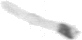
\includegraphics[height=2cm]{Preprocess/nonoise1}}%
  \hspace{2em}%
  \subcaptionbox{原图像的二值图\label{fig:nonoise2}}
      {
\includegraphics[height=2cm]{Preprocess/nonoise2}}\\
      ~\newline
  %\hspace{2em}%
  \subcaptionbox{预处理后的二值图\label{fig:nonoise3}}
      {
\includegraphics[height=2cm]{Preprocess/nonoise3}}
  \hspace{2em}%
  \subcaptionbox{预处理后的图像\label{fig:nonoise4}}
      {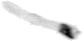
\includegraphics[height=2cm]{Preprocess/nonoise4}}
  \caption{图像预处理}
  \label{fig:nonoise}
\end{figure}

2、特征提取

采用~\ref{sec:FeatureExtraction}章节中提到特征描述方法对浮游生物的形态特征进行提取,可以实现从纹理、形状、灰度等不同角度对浮游生物形态特征进行描述。在特征提取后可以将提取的特征分为10类(每种特征提取方法提取的特征作为一类,其中粒子测度采用两组参数可以得到两组特征,将这两组特征分别作为一类),如图~\ref{fig:framework}所示。

3、特征选择

 在上一步中从不同角度提取了丰富的特征对浮游生物进行描述,然而这些特征中可能存在冗余或不相关的部分,它们不仅对分类性能的提高没有积极作用,甚至还会影响分类效率。因此,使用特征选择从所有特征中选取最优子集、去除冗余部分,可以提高分类的性能和效率。并且,对不同数据集进行分类时,采用特征选择可以针对每一个数据集从所有特征中找到适合的特征组合。本文采用了基于封装式评价准则的特征选择方法~\cite{Kohavi1997Wrappers},针对特征提取部分获得的10类特征分别进行选择,如图~\ref{fig:framework}所示。

4、多核学习

针对特征提取和特征选择后得到的10组特征信息,为每组特征分别选定3种核函数,采用多核学习的方法通过融合核函数实现特征的融合。在本文中使用非线性多核学~\cite{cortes2009learning}将所有核函数融合到一起,同时训练得到最终分类器,如图~\ref{fig:framework}所示。最终得到的分类器可以对未知的浮游生物图像进行识别,并具有广泛的适用范围和较高的准确率。下面设计对比实验对分类系统的性能进行评价。

\begin{figure}[H] % use float package if you want it here
  \centering
  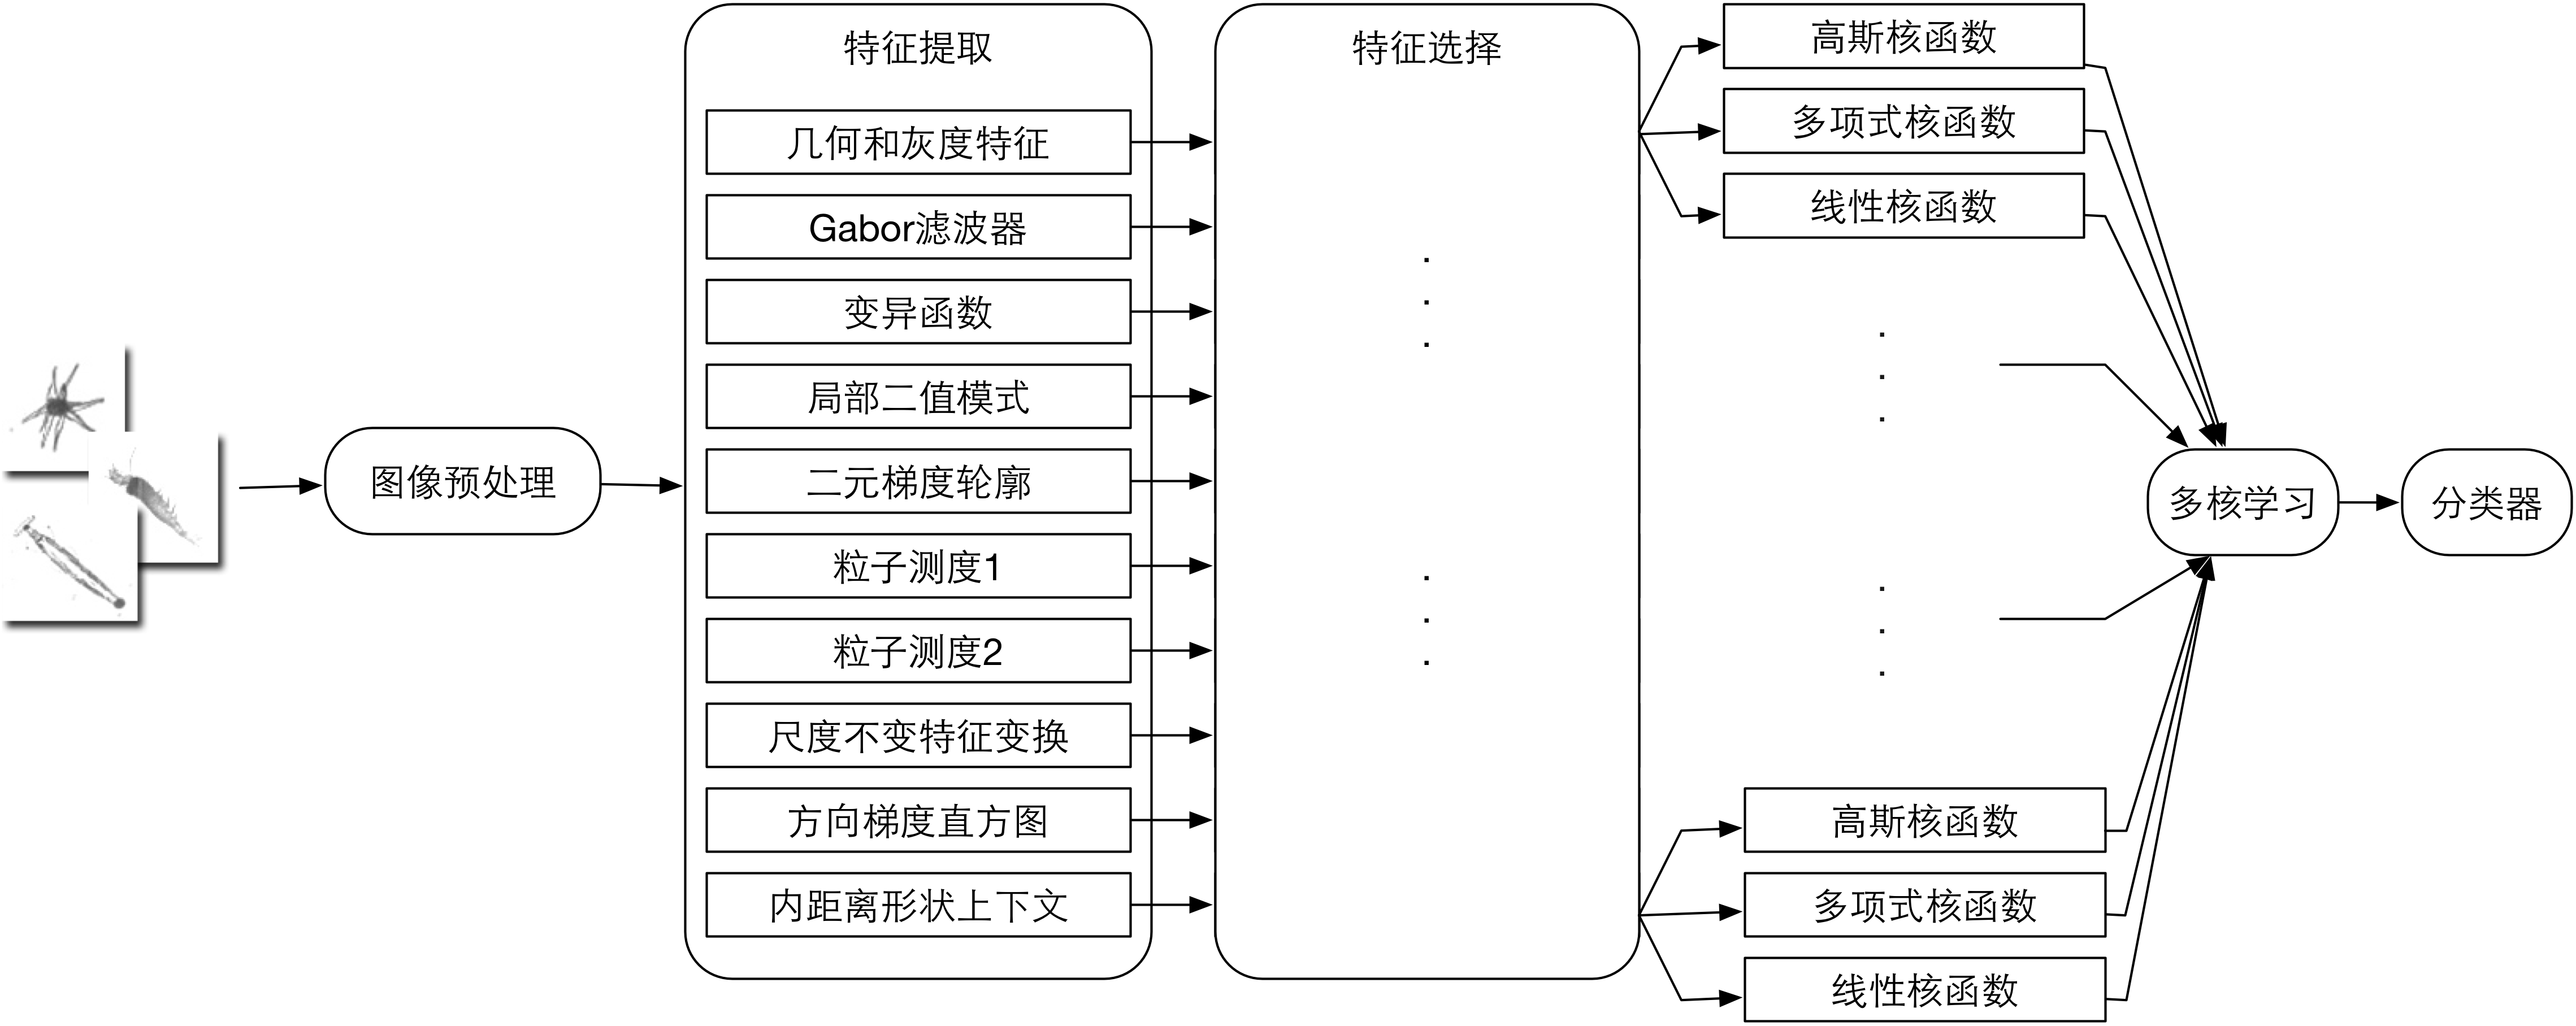
\includegraphics[height=6cm]{frame/framework}
  \caption{基于多核学习的浮游生物分类系统详细算法流程}
  \label{fig:framework}
\end{figure}

\section{对比实验}
\label{sec:experiment}

为了对本文设计的浮游生物分类系统的性能进行分析和评价,我们设计了如下三组对比实验:实验一是结合目前分类性能较好的浮游生物分类方法设计一个基准分类系统,作为分类系统性能对比评价的基准;实验二是在实验一的基础上,将使用~\ref{sec:FeatureExtraction}中提到的特征提取方法来对浮游生物特征进行描述;实验三采用本文设计的基于多核学习的浮游生物分类系统进行实验。将以上三个实验进行对比分析,从而实现对浮游生物分类系统各部分性能的评价。

\subsection{基准实验}
\label{sec:baselineExperiment}

根据Sosik等人在2007年提出的浮游植物自动分类方法~\cite{sosik2007automated}和ZooScan系统~\cite{gorsky2010digital}设计浮游生物分类的基准系统,该基准系统的算法流程框图如图\ref{fig:shiyan1frame}所示。
\begin{figure}[H] % use float package if you want it here
  \centering
  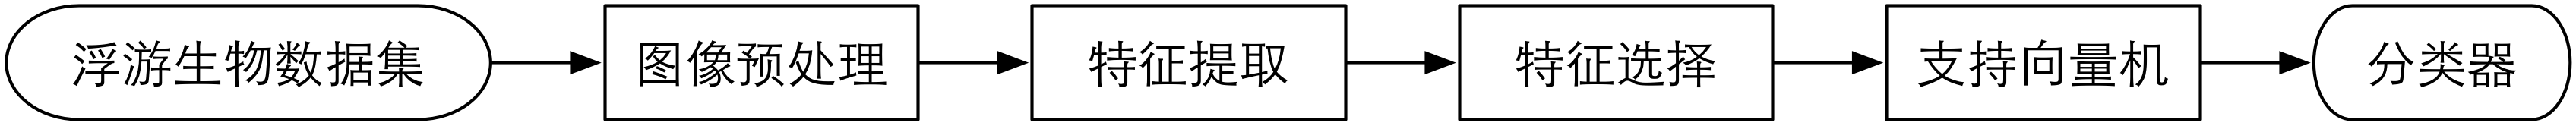
\includegraphics[height=0.7cm]{shiyan/shiyan1/shiyan1}
  \caption{基准实验的算法流程框图}
  \label{fig:shiyan1frame}
\end{figure}

首先对浮游生物图像进行预处理,降低图像中的噪声信息。然后对浮游生物形态特征进行提取,这里使用的特征提取方法结合了Sosik论文中的210个特征和ZooScan系统中的53个特征,因此经过特征提取每幅图像可以获得一个263维的特征向量。在得到每幅图像的特征后,采用特征选择除去其中的冗余部分。经过特征选择后,三个数据集保留下来的特征维数如表~\ref{tab:weishu}所示。最后对保留的特征归一化,用支持向量机算法来训练分类器,并使用混淆矩阵统计实验结果和分类准确率。

\begin{table}[htbp]
\small
  \centering
  \caption{特征选择后得到的特征维数}
  \label{tab:weishu}
  \begin{tabular}[c]{cccc}
    \toprule
    %\hline
    ~ & WHOI数据集 & ZooScan数据集 & Kaggle数据集\\
    \midrule
    %\hline
    特征维数 & 90 & 88 & 100\\
    \bottomrule
    %\hline
  \end{tabular}
\end{table}

该实验在~\ref{sec:dataset}中介绍的三个数据集上得到结果如表~\ref{tab:shiyan1Result}所示,混淆矩阵如图~\ref{fig:shiyan1}(图中横轴和纵轴为数据集中浮游生物的种类,见附录~\ref{fulu};图中数值表示分为对应类别图像的数量,数值越大颜色越深)。在WHOI采集的数据集上分类结果的F-Measure为0.8832,比相同条件下Sosik论文~\cite{sosik2007automated}中的分类结果有所提高。在ZooScan系统采集的数据集上得到分类结果的F-Measure为0.8212,相比于ZooScan系统的分类结果(0.7947)~\cite{gorsky2010digital}有一定提高。由此可以看出该实验设计的基准分类方法有较好的分类性能,可以作为评价浮游生物分类性能的基准。

\begin{figure}[h]
  \centering%
  \subcaptionbox{WHOI采集的数据集\label{fig:shiyan1whoiCM}}%标题的长度,超过则会换行,如下一个小图。
    {\includegraphics[height=5.5cm]{shiyan/shiyan1/whoiCM}}%\\%
  %~\newline
  %\hspace{2em}%
  \subcaptionbox{ZooScan采集的数据集\label{fig:shiyan1zooscanCM}}
      {\includegraphics[height=6cm]{shiyan/shiyan1/zooscanCM}}\\
  ~\newline
  %\hspace{2em}%
  \subcaptionbox{Kaggle竞赛数据集\label{fig:shiyan1kaggleCM}}
      {\includegraphics[height=11cm]{shiyan/shiyan1/kaggleCM}}
  \caption{基准实验分类结果的混淆矩阵}
  \label{fig:shiyan1}
\end{figure}

\begin{table}[htbp]
\small
  \centering
  \caption{基准实验的分类结果}
  \label{tab:shiyan1Result}
  \begin{tabular}[c]{cccc}
    \toprule
    %\hline
    ~ & WHOI数据集 & ZooScan数据集 & Kaggle数据集\\
    \midrule
    %\hline
    Recall & 0.8827 & 0.8060 & 0.7536\\
    %\hline
    %1-Precision & 11.63\% & 16.3\% & 21.49\%\\
    Precision & 0.8837 & 0.8370 & 0.7851\\
    F-Measure & 0.8832 & 0.8212 & 0.7690\\
    \bottomrule
    %\hline
  \end{tabular}
\end{table}

\subsection{特征对比实验}
\label{sec:featureexperiment}

在基准系统的基础上设计特征对比实验,使用~\ref{sec:FeatureExtraction}中的特征提取方法来对浮游生物进行描述,从而对本文设计分类系统的特征提取部分的性能进行评价,该实验的基本算法流程如图~\ref{fig:shiyan2frame}。
\begin{figure}[htbp] % use float package if you want it here
  \centering
  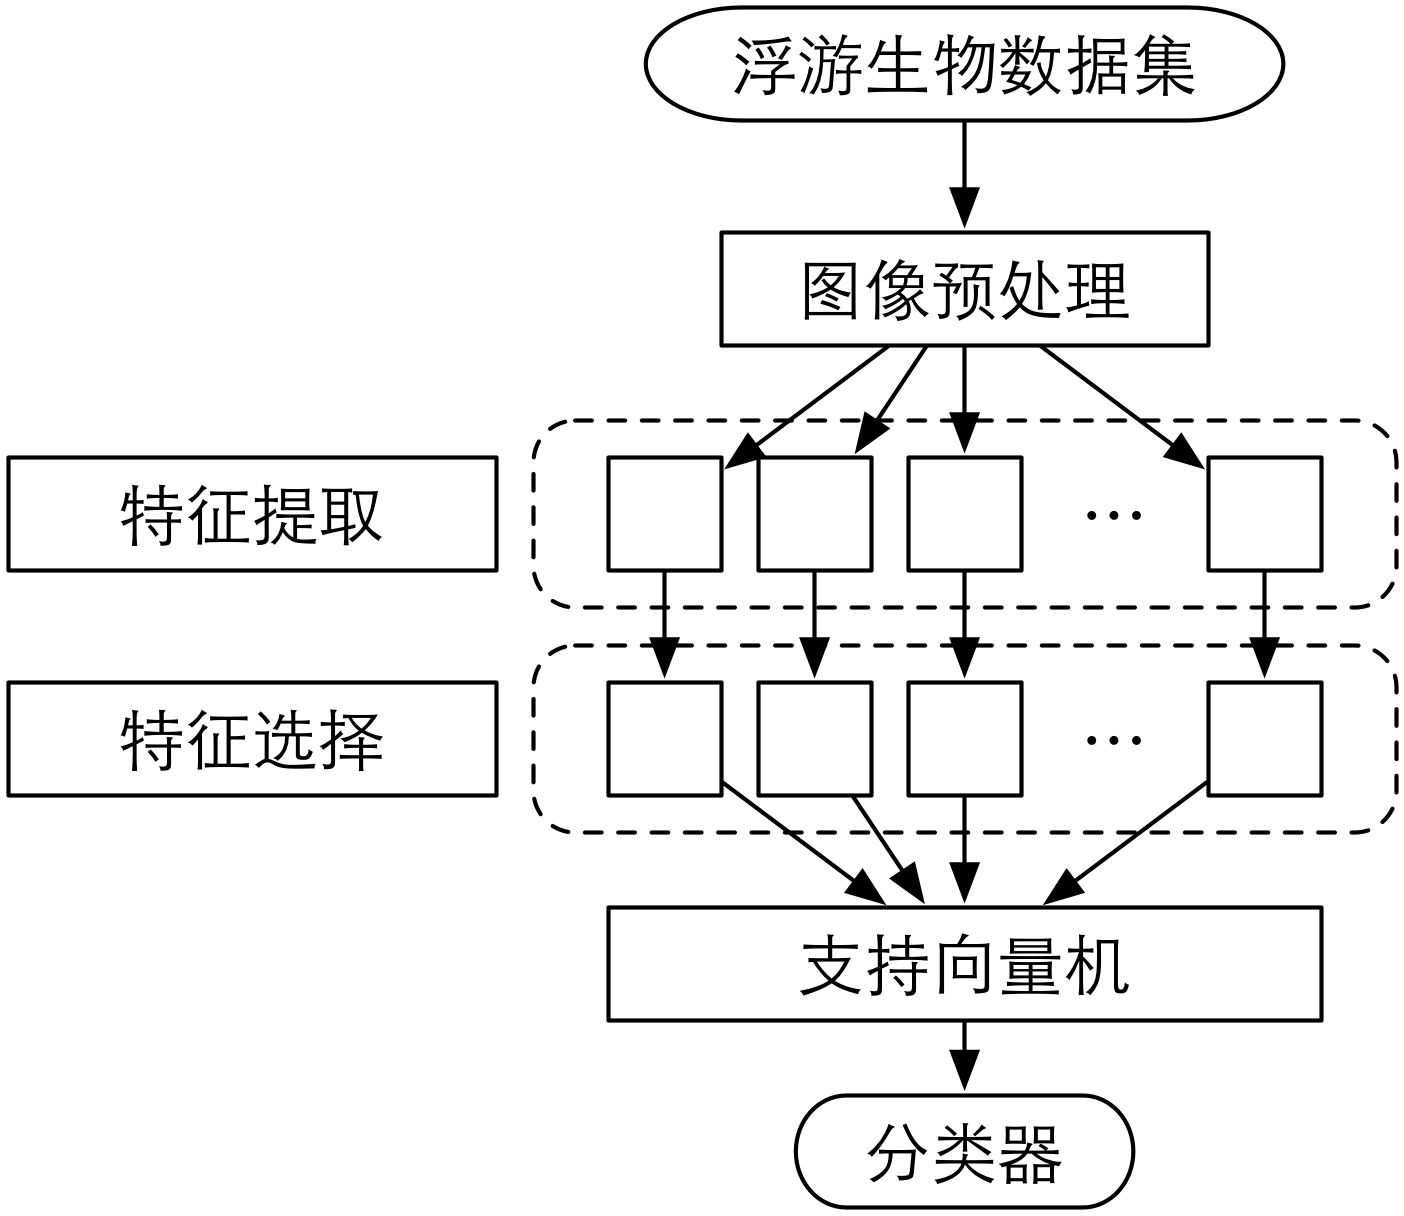
\includegraphics[height=6cm]{frame/jishu}
  \caption{特征对比实验算法流程框图}
  \label{fig:shiyan2frame}
\end{figure}

首先进行图像预处理,然后采用~\ref{sec:FeatureExtraction}中的特征提取方法分别提取浮游生物的形状、纹理等特征。在完成特征提取后,将所有特征分为10类(每类特征提取方法提取得到的特征作为一类,其中粒子测度采用两组参数提取特征得到两组特征)。针对每类特征分别采用特征选择方法去除冗余特征,然后将经过特征选择后的到的所有特征串联在一起,用支持向量机训练得到最终的分类器。

在三个数据集上进行实验时,支持向量机采用不同参数得到的分类结果如表~\ref{tab:shiyan2Result}所示。从表~\ref{tab:shiyan2Result}中能够得到,本实验在三个数据集上得到的最优分类结果及其相应的参数为:当采用高斯核函数且惩罚因子C=100时在WHOI取得最好分类结果,对应的F值为0.8963;在ZooScan系统采集的数据集上,当使用高斯核函数且C=10时取得最优分类结果,F值为0.8609;在Kaggle数据集上进行实验时采用高斯核函数且C=10取得最优分类结果,F值为0.8304。本实验在这三个数据集上取得的最优分类结果的混淆矩阵如图~\ref{fig:shiyan2}所示(图中横轴和纵轴为数据集中浮游生物的种类,见附录~\ref{fulu};图中数值表示分为对应类别图像的数量,数值越大颜色越深)。将实验结果与实验一的结果进行对比可以对本文设计的浮游生物分类系统的特征提取部分的性能进行评价。
%Recall = 89.57\%, 1-Precision = 10.3\%;Recall = 85.39\%, 1-Precision = 13.2\%;为Recall = 82.41\%, 1-Precision = 16.33\%

\begin{table}[htbp]
\scriptsize
  \centering
  \caption{特征对比实验的分类结果}
  \label{tab:shiyan2Result}
  \begin{tabular}[c]{ccccccccccc}
    \toprule
    %\hline
    \multirow{2}*{数据集} & \multirow{2}*{C} & \multicolumn{3}{c}{高斯核函数} & \multicolumn{3}{c}{多项式核函数} & \multicolumn{3}{c}{线性核函数}\\
    %\cline{3-8}
     & & Recall & Precision & F-Measure & Recall & Precision & F-Measure & Recall & Precision & F-Measure\\
    \midrule
    %\hline
    \multirow{3}*{WHOI数据集} & 1 & 0.8400 & 0.8457 & 0.8428 & 0.8897 & 0.8905 & 0.8901 & 0.8645 & 0.8659 & 0.8652\\
    %\cline{2-8}
     & 10 & 0.8894 & 0.8900 & 0.8897 & 0.8945 & 0.8953 & 0.8949 & 0.8812 & 0.8822 & 0.8817\\
    %\cline{2-8}
     & 100 & 0.8957 & 0.8970 & 0.8963 & 0.8842 & 0.8854 & 0.8848 & 0.8633 & 0.8641 & 0.8637\\
    \midrule
    %\hline
    \multirow{3}*{ZooScan数据集} & 1 & 0.7965 & 0.8394 & 0.8174 & 0.8245 & 0.8401 & 0.8322 & 0.7991 & 0.8186 & 0.8087\\
    %\cline{2-8}
     & 10 & 0.8539 & 0.8680 & 0.8609 & 0.8414 & 0.8478 & 0.8446 & 0.8552 & 0.8399 & 0.8475\\
    %\cline{2-8}
     & 100 & 0.8487 & 0.8638 & 0.8562 & 0.8304 & 0.8398 & 0.8351 & 0.8227 & 0.8177 & 0.8202\\
    \midrule
    %\hline
    \multirow{3}*{Kaggle数据集} & 1 & 0.7726 & 0.8104 & 0.7910 & 0.7748 & 0.8040 & 0.7891 & 0.7132 & 0.7491 & 0.7307\\
    %\cline{2-8}
     & 10 & 0.8241 & 0.8367 & 0.8304 & 0.8070 & 0.8192 & 0.8131 & 0.7844 & 0.7937 & 0.7890\\
    %\cline{2-8}
     & 100 & 0.8209 & 0.8311 & 0.826 & 0.7901 & 0.8027 & 0.7964 & 0.7810 & 0.7795 & 0.7802\\
    \bottomrule
    %\hline
  \end{tabular}
\end{table}

\begin{figure}[h]
  \centering%
  \subcaptionbox{WHOI采集的数据集\label{fig:shiyan2whoiCM}}
    {\includegraphics[height=5.3cm]{shiyan/shiyan2/whoiCM}}
  \subcaptionbox{ZooScan采集的数据集\label{fig:shiyan2zooscanCM}}
      {\includegraphics[height=5.8cm]{shiyan/shiyan2/zooscanCM}}\\
  ~\newline
  %\hspace{2em}%
  \subcaptionbox{Kaggle竞赛数据集\label{fig:shiyan2kaggleCM}}
      {\includegraphics[height=11cm]{shiyan/shiyan2/kaggleCM}}
  \caption{特征对比实验最优分类结果的混淆矩阵}
  \label{fig:shiyan2}
\end{figure}

\subsection{基于多核学习的浮游生物图像分类实验}
\label{sec:ourExperiment}

将本文提出的基于多核学习的浮游生物分类系统分别在三个数据集上进行实验。在实验中为了对多核学习的性能进行分析,针对多核学习算法中的核函数种类设计了两组实验:(1)在多核学习时,每种特征只设定一种核函数,其算法流程如图~\ref{fig:shiyan31}所示,该组实验使用不同核函数和参数得到的分类结果如表~\ref{tab:shiyan31Result}所示;(2)每种特征使用三种核函数(分别为高斯核函数、多项式核函数、线性核函数),该实验的算法流程图如图~\ref{fig:shiyan32}所示,不同参数得到的分类结果如表~\ref{tab:shiyan32Result}。

\begin{figure}
\begin{minipage}{0.48\textwidth}
  \centering
  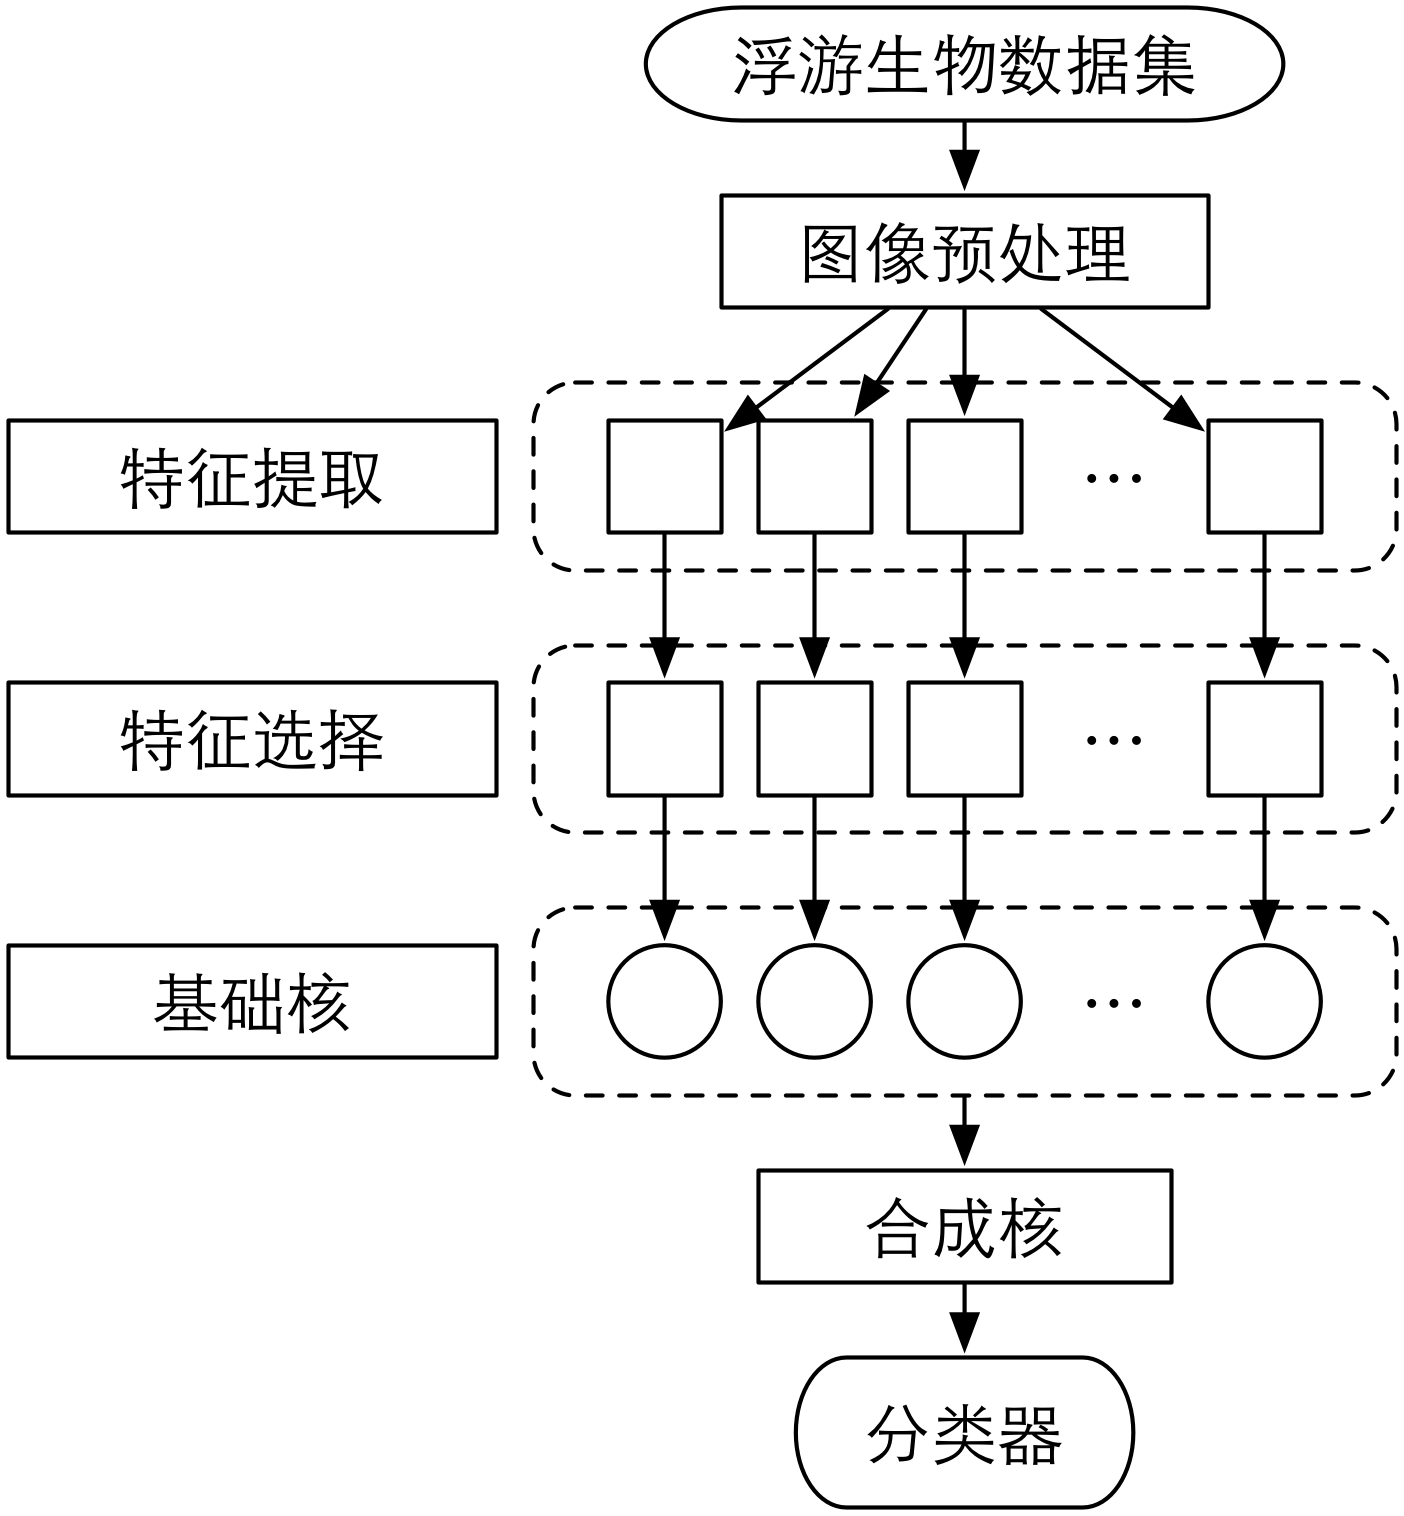
\includegraphics[height=6cm]{shiyan/shiyan3/shiyan31}
  \caption{基于多核学习的浮游生物分类的算法流程图(一种核函数)}
  \label{fig:shiyan31}
\end{minipage}\hfill
\begin{minipage}{0.48\textwidth}
  \centering
  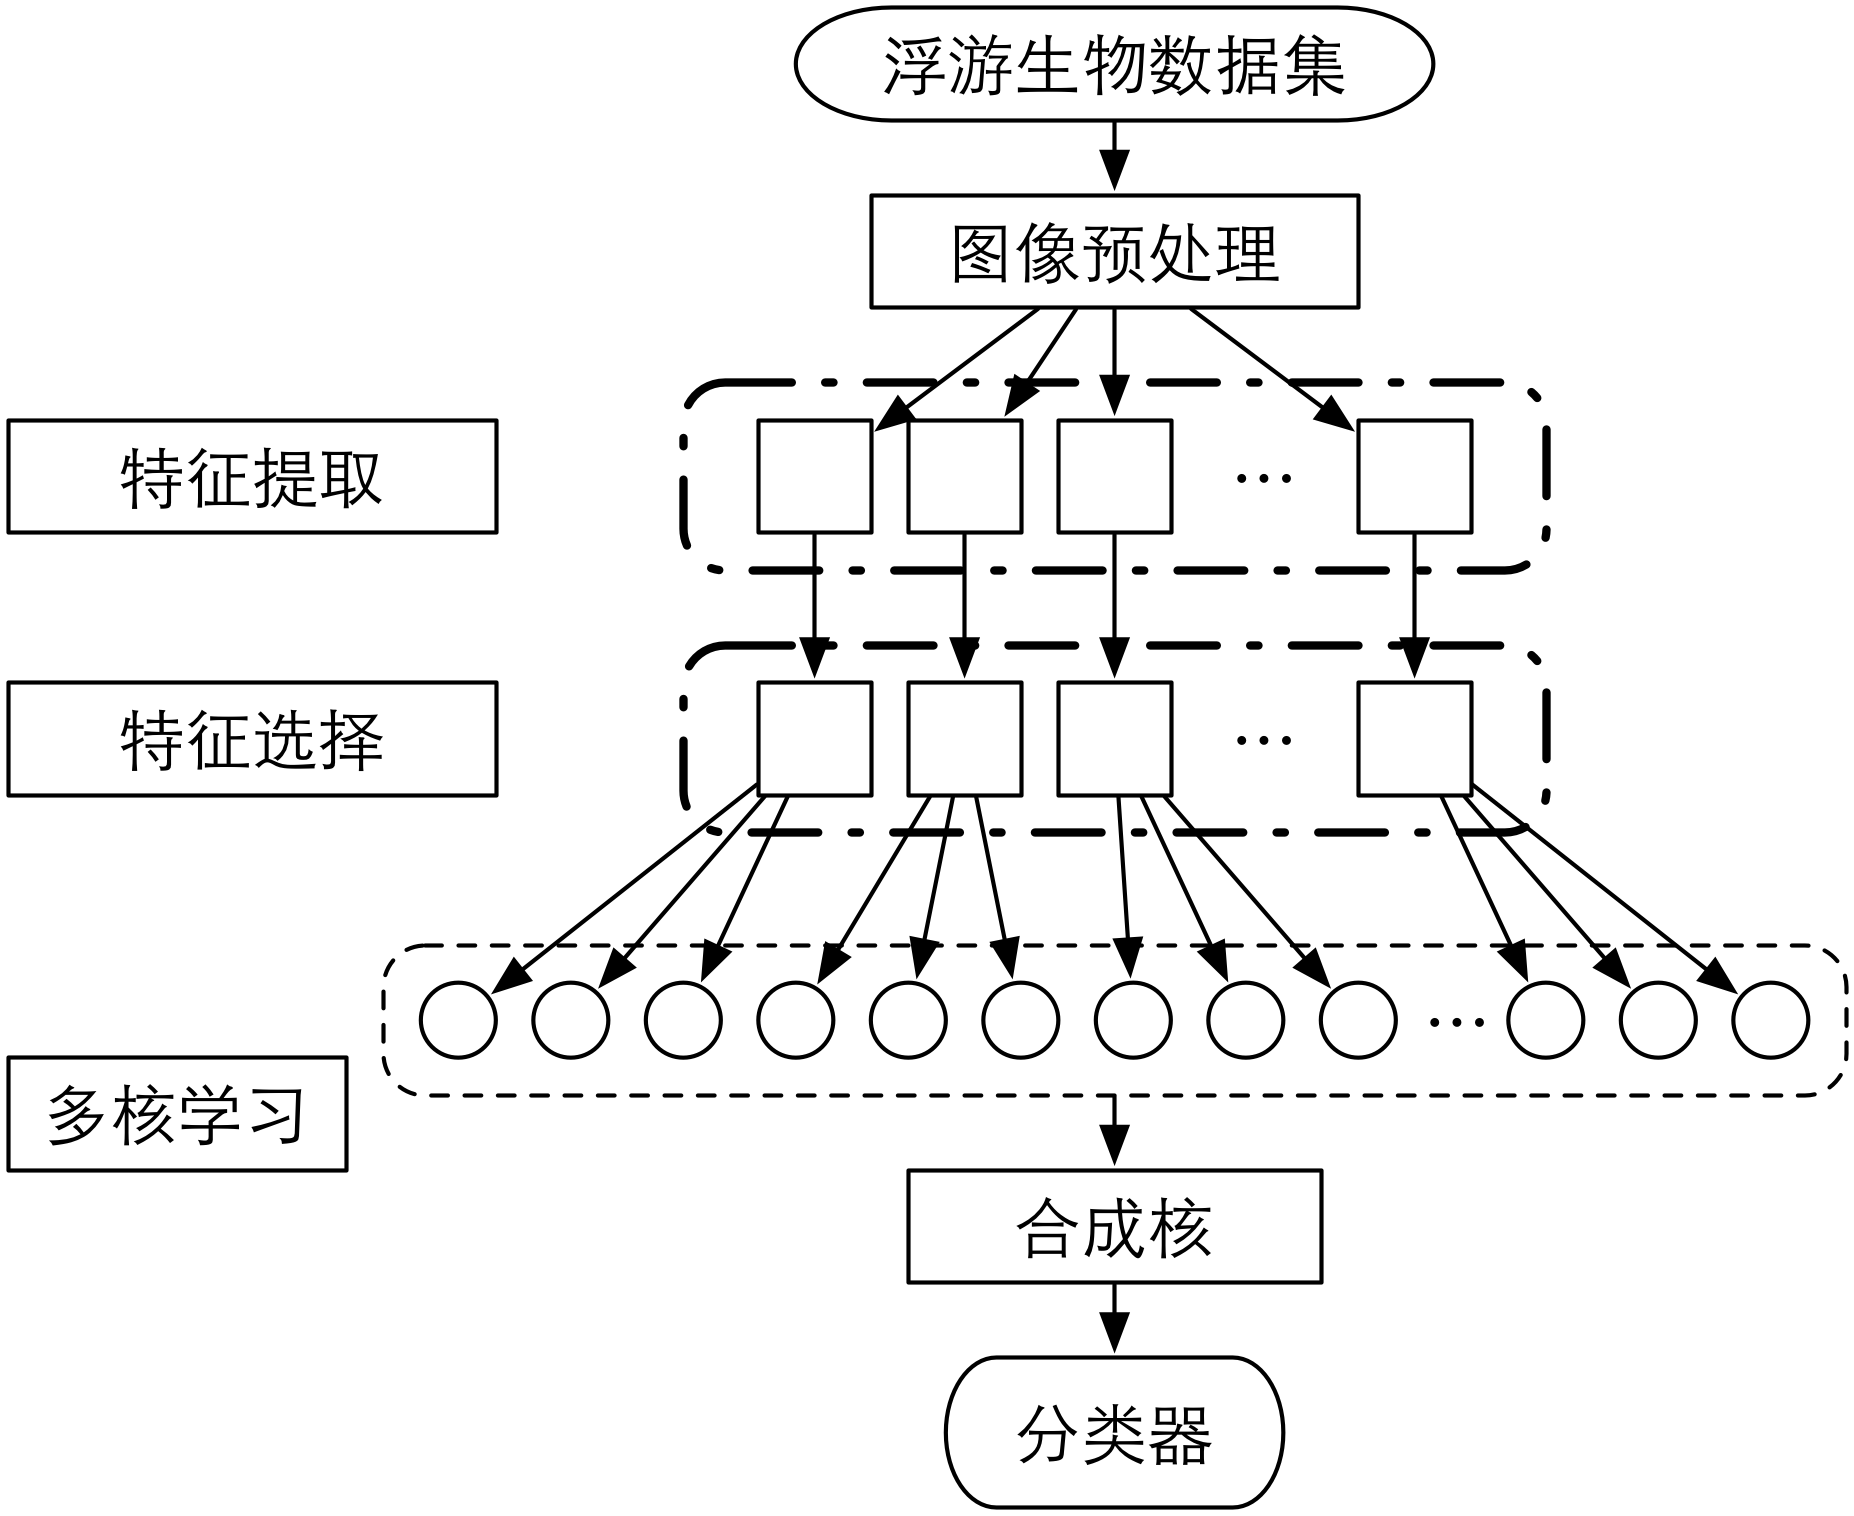
\includegraphics[height=6cm]{shiyan/shiyan3/shiyan32}
  \caption{基于多核学习的浮游生物分类的算法流程图(三种核函数)}
  \label{fig:shiyan32}
\end{minipage}
\end{figure}

\begin{table}[htbp]
\scriptsize
  \centering
  \caption{基于多核学习的浮游生物分类结果(一种核函数)}
  \label{tab:shiyan31Result}
  \begin{tabular}[c]{ccccccccccc}
    \toprule
    %\hline
    \multirow{2}*{数据集} & \multirow{2}*{C} & \multicolumn{3}{c}{高斯核函数} & \multicolumn{3}{c}{多项式核函数} & \multicolumn{3}{c}{线性核函数}\\
    %\cline{3-8}
     & & Recall & 1-Precision & F-Measure & Recall & 1-Precision & F-Measure & Recall & 1-Precision & F-Measure\\
    \midrule
    %\hline
    \multirow{3}*{WHOI数据集} & 1 & 0.8848 & 0.8865 & 0.8856 & 0.8958 & 0.8979 & 0.8968 & 0.8855 & 0.8882 & 0.8868\\
    %\cline{2-8}
     & 10 & 0.8875 & 0.8896 & 0.8885 & 0.8967 & 0.8984 & 0.8975 & 0.8912 & 0.8935 & 0.8923\\
    %\cline{2-8}
     & 100 & 0.8858 & 0.8880 & 0.8869 & 0.8939 & 0.8956 & 0.8947 & 0.8842 & 0.8859 & 0.8850\\
    \midrule
    %\hline
    \multirow{3}*{ZooScan数据集} & 1 & 0.8332 & 0.8826 & 0.8572 & 0.8394 & 0.8739 & 0.8553 & 0.8178 & 0.8447 & 0.8310\\
    %\cline{2-8}
     & 10 & 0.8626 & 0.8999 & 0.8809 & 0.8674 & 0.8824 & 0.8748 & 0.8398 & 0.8472 & 0.8435\\
    %\cline{2-8}
     & 100 & 0.8660 & 0.9008 & 0.8831 & 0.8679 & 0.8837 & 0.8757 & 0.8351 & 0.8437 & 0.8394\\
    \midrule
    %\hline
    \multirow{3}*{Kaggle数据集} & 1 & 0.7846 & 0.8259 & 0.8047 & 0.8039 & 0.8324 & 0.8179 & 0.7809 & 0.8076 & 0.7940\\
    %\cline{2-8}
     & 10 & 0.8295 & 0.8358 & 0.8326 & 0.8260 & 0.8438 & 0.8348 & 0.8132 & 0.8234 & 0.8183\\
    %\cline{2-8}
     & 100 & 0.8297 & 0.8316 & 0.8306 & 0.8211 & 0.8418 & 0.8313 & 0.7968 & 0.8090 & 0.8029\\
    \bottomrule
    %\hline
  \end{tabular}
\end{table}

\begin{table}[htbp]
\scriptsize
  \centering
  \caption{基于多核学习的浮游生物分类结果(三种核函数)}
  \label{tab:shiyan32Result}
  \begin{tabular}[c]{ccccc}
    \toprule
    %\hline
    \multirow{2}*{数据集} & \multirow{2}*{C} & \multicolumn{3}{c}{高斯核函数+多项式核函数+线性核函数}\\
    %\cline{3-4}
     & & Recall & 1-Precision & F-Measure\\
    \midrule
    %\hline
    \multirow{3}*{WHOI数据集} & 1 & 0.8964 & 0.8983 & 0.8973\\
    %\cline{2-4}
     & 10 & 0.8988 & 0.8997 & 0.8992\\
    %\cline{2-4}
     & 100 & 0.9000 & 0.9009 & 0.9004\\
    \midrule
    %\hline
    \multirow{3}*{ZooScan数据集} & 1 & 0.8542 & 0.8862 & 0.8699\\
    %\cline{2-4}
     & 10 & 0.8834 & 0.9042 & 0.8937\\
    %\cline{2-4}
     & 100 & 0.8831 & 0.9019 & 0.8924\\
    \midrule
    %\hline
    \multirow{3}*{Kaggle数据集} & 1 & 0.8030 & 0.8388 & 0.8205\\
    %\cline{2-4}
     & 10 & 0.8367 & 0.8551 & 0.8458\\
    %\cline{2-4}
     & 100 & 0.8346 & 0.8512 & 0.8428\\
    \bottomrule
    %\hline
  \end{tabular}
\end{table}

根据表~\ref{tab:shiyan31Result}能够发现,采用一种核函数在三个数据集上取得的最优分类结果为:在WHOI数据集上进行实验,采用多项式核函数且C = 10时得到的最优结果,F值为0.8975;在ZooScan采集的数据集上,采用高斯核函数且C=100时取得最优分类结果,F值为0.8831;在kaggle数据集上取得最优分类结果的F值为0.8348,对应的参数为多项式核函数且C=10。图~\ref{fig:shiyan3}为以上最优分类结果对应的混淆矩阵(图中横轴和纵轴为数据集中浮游生物的种类,见附录~\ref{fulu};图中数值表示分为对应类别图像的数量,数值越大颜色越深)。分析表~\ref{tab:shiyan32Result}可以得到使用三种核函数在三个数据集上的最优分类结果:WHOI数据集F值为0.9004;ZooScan数据集F值为0.8937;Kaggle数据集F值为0.8458。将本实验与之前的实验结果进行对比可以对基于多核学习的浮游生物分类系统的整体性能进行评价。
%Recall = 89.6\%, 1-Precision = 10.16\%;为Recall = 86.79\%, 1-Precision = 11.63\%;Recall = 82.6\%, 1-Precision = 15.62\%;
%Recall = 90\%,1-Precsion = 9.91\%;Recall = 88.34\%,1-Precision = 9.58\%;Recall = 83.67\%,1-Precision = 14.49\%

\begin{figure}[h]
  \centering%
  \subcaptionbox{WHOI采集的数据集\label{fig:shiyan3whoiCM}}%标题的长度,超过则会换行,如下一个小图。
    {\includegraphics[height=5.5cm]{shiyan/shiyan3/whoiCM}}%\\%
  %~\newline
  %\hspace{2em}%
  \subcaptionbox{ZooScan采集的数据集\label{fig:shiyan3zooscanCM}}
      {\includegraphics[height=6cm]{shiyan/shiyan3/zooscanCM}}\\
  ~\newline
  %\hspace{2em}%
  \subcaptionbox{Kaggle竞赛数据集\label{fig:shiyan3kaggleCM}}
      {\includegraphics[height=11cm]{shiyan/shiyan3/kaggleCM}}
  \caption{基于多核学习的浮游生物最优分类结果的混淆矩阵(一种核函数)}
  \label{fig:shiyan3}
\end{figure}

\section{实验结果分析}

浮游生物包括浮游植物和动物两大类,这两类生物之间的形态差别较大。同时,浮游生物的种类繁多,按照“界门纲目科属种”的级别进行划分,从“界”到“种”,越向下被归为同一属的生物之间形态相差越小。以上这两个方面是浮游生物分类研究两个较大的难点。为了扩大浮游生物分类系统的适用范围,提高分类的准确率,我们提出了一种基于多核学习的浮游生物分类系统,该系统具有以下特点:首先,从多个角度对浮游生物的特征进行描述,具有较广的适用范围;其次,采用特征选择算法去除冗余特征;最后使用多核学习训练分类器,提高分类器的性能。

为了对本文提出的系统性能进行评价,在\ref{sec:experiment}中设计了三组对比实验。实验一为基准实验,综合目前性能较好的浮游生物分类方法设计而来,作为评价分类系统对比的基准。实验二是在实验一的基础上使用\ref{sec:FeatureExtraction}中的方法提取浮游生物特征,通过对比实验一与实验二的分类结果对特征提取方法的性能进行评价。实验三将本文设计的浮游生物分类系统在三个数据集上进行实验,将其分类结果与实验一和二对比来对分类系统总体性能进行评价。

根据表~\ref{tab:shiyan1Result}和表~\ref{tab:shiyan2Result},比较实验一与实验二在三个数据集上取得的最优分类结果可得表~\ref{tab:compare1and2}。从表~\ref{tab:compare1and2}中能够得出,实验二在三个数据集上取得的分类准确率比实验一都有一定程度的提高,同时错误率也相应的降低,其中在Kaggle数据集上的效果最为明显,F值提高了0.0641,分类性能有明显提高。此外,对比图~\ref{fig:shiyan1}和图~\ref{fig:shiyan2}可以看出:与实验一相比,实验二得到的分类结果,在Kaggle竞赛数据集上有36个类别的准确提高了,在WHOI和ZooScan采集的数据集上分别有14、16个类别提高。由此可以看出,结合多种特征对浮游生物的形态特征进行全面描述有利浮游生物的区分。例如,图~\ref{fig:shiyan1zooscanCM}中“Appendicularia”类图像中有58张图在实验一中被错误的分为“Gelatinous\_sipho\_cloche”类,而在实验二中,这个数字从58下降到了10。因此,在分类过程中从多个角度的对浮游生物的形态特征进行描述,可以提高分类系统的性能。

\begin{table}[htbp]
\small
  \centering
  \caption{特征对比实验与基准实验分类结果的对比}
  \label{tab:compare1and2}
  \begin{tabular}[c]{cc}
    \toprule
    %\hline
    数据集 & F-Measure提高量\\
    \midrule
    %\hline
    WHOI数据集 & 0.0131\\
    %\hline
    ZooScan数据集 & 0.0397\\
    %\hline
    Kaggle数据集 & 0.0641\\
    \bottomrule
    %\hline
  \end{tabular}
\end{table}

% \begin{table}[htbp]
%   \centering
%   \caption{实验二与实验一分类结果的对比}
%   \label{tab:compare1and2}
%   \begin{tabular}[c]{ccc}
%     \toprule
%     %\hline
%     数据集 & Recall & 1-Precision\\
%     \midrule
%     %\hline
%     WHOI数据集 & 1.3\% & -1.33\%\\
%     %\hline
%     ZooScan数据集 & 4.79\% & -3.1\%\\
%     %\hline
%     Kaggle数据集 & 7.05\% & -5.16\%\\
%     \bottomrule
%     %\hline
%   \end{tabular}
% \end{table}

实验三包含了两组实验:一个是在多核学习过程中每种特征只选用一种核函数;另一个是在多核学习时每种特征使用三种核函数。对比表~\ref{tab:shiyan31Result}和表~\ref{tab:shiyan2Result}中最优分类准确率可以的表~\ref{tab:compare31and2},这是实验三中每种特征使用一种核函数的多核学习与实验二的对比结果,可以得出使用多核学习能够提高分类器的性能。观察混淆矩阵图~\ref{fig:shiyan2}和图~\ref{fig:shiyan3}可以发现:采用多核学习得到的分类结果,在WHOI采集的数据集中有11类图像分类结果得到了提高,在Kaggle数据集上有21类,而在ZooScan数据集上所有类别的准确率都得到了提高。由此可见,采用多核学习的分类系统相较于采用单核学习方法的分类系统有较好的性能。同时,对比表~\ref{tab:shiyan31Result}和~\ref{tab:shiyan32Result}得到表~\ref{tab:compare3},可以发现使用多核学习时每种特征采用三种不同的核函数会使分类准确率有进一步的提高。

\begin{table}[htbp]
\small
  \centering
  \caption{基于多核学习的浮游生物分类实验(一种核函数)与特征对比实验分类结果对比}
  \label{tab:compare31and2}
  \begin{tabular}[c]{cc}
    \toprule
    %\hline
    数据集 & F-Measure提高量\\
    \midrule
    %\hline
    WHOI数据集 & 0.0012\\
    %\hline
    ZooScan数据集 & 0.0122\\
    %\hline
    Kaggle数据集 & 0.0044\\
    \bottomrule
    %\hline
  \end{tabular}
\end{table}

% \begin{table}[htbp]
%   \centering
%   \caption{每种特征使用一种核函数得到的分类结果与实验二分类结果的对比}
%   \label{tab:compare31and2}
%   \begin{tabular}[c]{ccc}
%     \toprule
%     %\hline
%     数据集 & Recall & 1-Precision\\
%     \midrule
%     %\hline
%     WHOI数据集 & 0.1\% & -0.14\%\\
%     %\hline
%     ZooScan数据集 & 1.4\% & -1.57\%\\
%     %\hline
%     Kaggle数据集 & 0.19\% & -0.71\%\\
%     \bottomrule
%     %\hline
%   \end{tabular}
% \end{table}

\begin{table}[htbp]
\small
  \centering
  \caption{每种特征使用三种核函数和一种核函数得到的分类结果对比}
  \label{tab:compare3}
  \begin{tabular}[c]{cc}
    \toprule
    %\hline
    数据集 & F-Measure提高量\\
    \midrule
    %\hline
    WHOI数据集 & 0.0029\\
    %\hline
    ZooScan数据集 & 0.0106\\
    %\hline
    Kaggle数据集 & 0.0110\\
    \bottomrule
    %\hline
  \end{tabular}
\end{table}

根据表~\ref{tab:shiyan32Result}可得,我们提出的基于多核学习的分类系统在三个数据集的上最优分类结果的F值可以达到0.9004、0.8937、0.8458,与实验一基准系统的最优分类结果对比有很大提高,如表~\ref{tab:compare3and1}。其中在Kaggle数据集上的性能提高最明显,F值提高了0.0768。有此可以看出,本文提出的基于多核学习的浮游生物分类系统有较好的分类性能和较高的泛化能力,可以广泛的应用于浮游生物研究。

\begin{table}[ht]
\small
  \centering
  \caption{基于多核学习的浮游生物分类实验(三种核函数)与基准实验分类结果对比}
  \label{tab:compare3and1}
  \begin{tabular}[c]{cc}
    \toprule
    %\hline
    数据集 & F-Measure提高量\\
    \midrule
    %\hline
    WHOI数据集 & 0.0172\\
    %\hline
    ZooScan数据集 & 0.0725\\
    %\hline
    Kaggle数据集 & 0.0768\\
    \bottomrule
    %\hline
  \end{tabular}
\end{table}

% \begin{table}[ht]
%   \centering
%   \caption{基于多核学习的浮游生物分类系统与基准系统的分类结果的对比}
%   \label{tab:compare3and1}
%   \begin{tabular}[c]{ccc}
%     \toprule
%     %\hline
%     数据集 & Recall & 1-Precision\\
%     \midrule
%     %\hline
%     WHOI数据集 & 1.73\% & -1.72\%\\
%     %\hline
%     ZooScan数据集 & 7.74\% & -6.72\%\\
%     %\hline
%     Kaggle数据集 & 8.31\% & -7\%\\
%     \bottomrule
%     %\hline
%   \end{tabular}
% \end{table}

\section{本章小结}

本文提出了基于多核学习的浮游生物分类系统,该系统主要采用多核学习融合多种特征进行分类识别,提高了分类系统的泛化能力和分类性能。本章介绍了多核学习的原理,采用非线性多核学习来进行特征融合和训练分类器。为了检验分类系统的分类性能,我们还设计了三组实验进行对比。首先根据Sosik等人提出的浮游植物分类系统~\cite{sosik2007automated}和ZooScan系统~\cite{gorsky2010digital}设计基准分类系统,以此作为后续实验对比的基准;其次还设计了特征对比实验,对分类系统中特征提取部分的性能进行评价;最后采用本文设计的浮游生物分类系统进实验,对该分类系统的性能进行评价分析。在设计对比实验的同时为了检验系统的泛化能力,将所有的实验都分别在三个不同的数据集上进行。
